\chapter{Specifikacija programske potpore}
		
	\section{Funkcionalni zahtjevi}
			
			%\textbf{\textit{dio 1. revizije}}\\
			
			%\textit{Navesti \textbf{dionike} koji imaju \textbf{interes u ovom sustavu} ili  \textbf{su nositelji odgovornosti}. To su prije svega korisnici, ali i administratori sustava, naručitelji, razvojni tim.}\\
				
			%\textit{Navesti \textbf{aktore} koji izravno \textbf{koriste} ili \textbf{komuniciraju sa sustavom}. Oni mogu imati inicijatorsku ulogu, tj. započinju određene procese u sustavu ili samo sudioničku ulogu, tj. obavljaju određeni posao. Za svakog aktora navesti funkcionalne zahtjeve koji se na njega odnose.}\\
			
			
			\noindent \textbf{Dionici:}
			
			\begin{packed_enum}
				
				\item Vlasnik
				\item Klijenti
				\begin{packed_enum}
					\item Organizatori
					\item Posjetitelji
				\end{packed_enum}				
				\item Administratori
				\item Razvojni tim
				
			\end{packed_enum}
			
			\noindent \textbf{Aktori i njihovi funkcionalni zahtjevi:}

			\begin{packed_enum}
				\item \underbar{Neregistrirani/neprijavljeni korisnik (inicijator) može:}
				
				\begin{packed_enum}
					
					\item prijaviti se u sustav, unijeti korisničko ime i lozinku
					\item registrirati se u sustav, stvoriti korisnički račun za koji su mu potrebni korisničko ime, lozinka i e-mail adresa

				\end{packed_enum}

				\item \underbar{Prijavljeni korisnik (inicijator) može:}
				
				\begin{packed_enum}
					
					\item pregledati popis događaja
					\item kontrolirati način prikaza popisa događaja
					\begin{packed_enum}
						\item filtrirati događaje po kategoriji, lokaciji, vremenu održavanja
						\item sortirati događaje po kategoriji, udaljenosti, vremenu održavanja, cijeni, ocjeni
						\item pretraživati događaje po ključnim riječima
					\end{packed_enum}
					\item pregledati detalje događaja
					\item pregledati recenzije drugih posjetitelja
					\item odjaviti se iz sustava
					\item pregledati osobne podatke
					\item uređivati osobne podatke
					\item izbrisati svoj korisnički račun
					\item pregledati javni profil pojedinog organizatora
				\end{packed_enum}

				\item  \underbar{Organizator (inicijator) može:}
				
				\begin{packed_enum}
					
					\item sve što prijavljeni korisnik može
					\item stvoriti novi događaj i dodati mu potrebne informacije (opis, lokacija, vremenski raspored, cijena)
					\item uređivati vlastiti postojeći događaj
					\begin{packed_enum}
						
						\item izmijeniti nužne informacije o događaju (opis, lokacija, vremenski raspored, cijena)
						\item dodati, obrisati ili izmijeniti izborne informacije o događaju (slika, kategorija i sl.)
						
					\end{packed_enum}
					\item izbrisati vlastiti postojeći događaj
					\item pregledati statistiku za vlastite događaje
					\item dobiti uvid u recenzije događaja koje je organizirao
					\item uređivati ili skriti vlastiti javni profil
					\item upravljati pretplatom za premium organizatore
					\begin{packed_enum}
						
						\item pretplatiti se kao premium organizator putem PayPal-a ili kreditne kartice
						\item ukinuti pretplatu
						
					\end{packed_enum}
				
				\end{packed_enum}

				\item \underbar{Posjetitelj (inicijator) može:}
				
				\begin{packed_enum}
					
					\item sve što prijavljeni korisnik može
					\item odabrati i/ili promijeniti stupanj interesa za događaj („sigurno dolazim“, „možda dolazim“, „ne dolazim“)
					\item ostaviti i urediti recenziju za posjećeni događaj koji je završio unutar zadnjih 48h (ocjena, komentar)
					
				\end{packed_enum}
			
				\item  \underbar{Administrator (inicijator) može:}
				
				\begin{packed_enum}
					
					\item sve što prijavljeni korisnik može
					\item vidjeti popis svih registriranih korisnika i njihovih osobnih podataka
					\item dodavati nove administratore
					\item pristupiti statistici o korištenju aplikacije
					\item ukloniti recenzije koje krše pravila korištenja aplikacije
					\item ukloniti događaje koji krše pravila korištenja aplikacije
					\item ukloniti korisničke račune koji krše pravila korištenja aplikacije
					\item ukinuti pretplatu premium organizatorima koji krše pravila korištenja aplikacije
					\item postaviti cijenu članstva za premium organizatore					
				\end{packed_enum}

				\item  \underbar{Baza podataka (sudionik):}
				
				\begin{packed_enum}
					
					\item pohranjuje sve podatke o korisnicima, njihovim detaljima i ovlastima
					\item pohranjuje sve podatke o događajima, njihovim detaljima i recenzijama
					
				\end{packed_enum}
			\end{packed_enum}
			
			\eject 
			
			
				
			\subsection{Obrasci uporabe}
				
				%\textbf{\textit{dio 1. revizije}}
				
				\subsubsection{Opis obrazaca uporabe}
					%\textit{Funkcionalne zahtjeve razraditi u obliku obrazaca uporabe. Svaki obrazac je potrebno razraditi prema donjem predlošku. Ukoliko u nekom koraku može doći do odstupanja, potrebno je to odstupanje opisati i po mogućnosti ponuditi rješenje kojim bi se tijek obrasca vratio na osnovni tijek.}\\
					

					\noindent \underbar{\textbf{UC1 -Registracija}}
					\begin{packed_item}

						\item \textbf{Glavni sudionik:} Korisnik
						\item  \textbf{Cilj:} Stvoriti korisnicki račun za pristup sustavu
						\item  \textbf{Sudionici:} Baza podataka
						\item  \textbf{Preduvjet:} 
						\item  \textbf{Opis osnovnog tijeka:}

						\item[] \begin{packed_enum}

							\item Korisnik odabire opciju za registraciju
							\item Korisnik unosi potrebne korisničke podatke
							\item Korisnik prima obavijest o uspješnoj registraciji 

						\end{packed_enum}

						\item  \textbf{Opis mogućih odstupanja:}

						\item[] \begin{packed_item}

							\item[2.a] Odabir vec zauzetog korisničkog imena i/ili e-maila, unos korisničkog podatka u nedozvoljenom formatu ili pruzanje neispravnoga e-maila 
							\item[] \begin{packed_enum}

								\item Sustav obavjestava korisnika o neuspjelom upisu i vraća ga na stranicu za registraciju
								\item Korisnik mijenja potrebne podatke te zavrsava unos ili odustaje od registracije

							\end{packed_enum}
						\end{packed_item}
					\end{packed_item}

					\noindent \underbar{\textbf{UC2 - Prijava}}
					\begin{packed_item}

						\item \textbf{Glavni sudionik:} Korisnik
						\item  \textbf{Cilj:} Dobiti pristup korisnickom sučelju
						\item  \textbf{Sudionici:} Baza podataka
						\item  \textbf{Preduvjet:} Registracija
						\item  \textbf{Opis osnovnog tijeka:}

						\item[] \begin{packed_enum}

							\item Unos korisničkog imena i lozinke
							\item Potvrda o ispravnosti unesenih podataka
							\item Pristup korisničkim funkcijama

						\end{packed_enum}

						\item  \textbf{Opis mogućih odstupanja:}

						\item[] \begin{packed_item}

							\item[2.a] Neispravno korisnicko ime/lozinka 
							\item[] \begin{packed_enum}

								\item Sustav obavjestava korisnika o neuspjelom upisu i vraća ga na stranicu za prijavu

							\end{packed_enum}

						\end{packed_item}
					\end{packed_item}


					\noindent \underbar{\textbf{UC3 - Pregled osobnih podataka}}
					\begin{packed_item}

						\item \textbf{Glavni sudionik:} Administrator, organizator, posjetitelj
						\item  \textbf{Cilj:} Pregledati osobne podatke
						\item  \textbf{Sudionici:} Baza podataka
						\item  \textbf{Preduvjet:} Korisnik je prijavljen
						\item  \textbf{Opis osnovnog tijeka:}

						\item[] \begin{packed_enum}

							\item Korisnik odabire opciju ”Osobni podatci”
							\item Aplikacija prikazuje osobne podatke korisnika

						\end{packed_enum}

					\end{packed_item}

					\noindent \underbar{\textbf{UC4 - Promjena osobnih podataka}}
					\begin{packed_item}

						\item \textbf{Glavni sudionik:} Organizator, posjetitelj
						\item  \textbf{Cilj:} Promijeniti osobne podatke
						\item  \textbf{Sudionici:} Baza podataka
						\item  \textbf{Preduvjet:} Organizator je prijavljen
						\item  \textbf{Opis osnovnog tijeka:}

						\item[] \begin{packed_enum}

							\item Korisnik odabere opciju za promjenu podataka
							\item Korisnik mijenja svoje osobne podatke
							\item Korisnik sprema promjene
							\item Baza podataka se ažurira

						\end{packed_enum}

						\item  \textbf{Opis mogućih odstupanja:}

						\item[] \begin{packed_item}

							\item[2.a] Korisnik promijeni svoje osobne podatke, ali ne odabere opciju ”Spremi
							promjenu”
							\item[] \begin{packed_enum}

								\item Sustav obavjestava korisnika da nije spremio podatke prije izlaska iz prozora

							\end{packed_enum}

						\end{packed_item}

					\end{packed_item}

					\noindent \underbar{\textbf{UC5 - Brisanje računa}}
					\begin{packed_item}

						\item \textbf{Glavni sudionik:} Administrator, korisnik
						\item  \textbf{Cilj:} Izbrisati svoj korisnički račun
						\item  \textbf{Sudionici:} Baza podataka
						\item  \textbf{Preduvjet:} Korisnik je prijavljen
						\item  \textbf{Opis osnovnog tijeka:}

						\item[] \begin{packed_enum}

							\item Korisnik pregledava osobne podatke
							\item Otvara se stranica s osobnim podacima korisnika
							\item Korisnik briše račun
							\item Korisnicki račun se izbriše iz baze podataka
							\item Otvara se stranica za registraciju
						\end{packed_enum}

						\item  \textbf{Opis mogućih odstupanja:}


					\end{packed_item}

					\noindent \underbar{\textbf{UC6 - Pregled popisa događaja}}
					\begin{packed_item}

						\item \textbf{Glavni sudionik:} Administrator, korisnik
						\item  \textbf{Cilj:} Pregledati nadolazeće događaje
						\item  \textbf{Sudionici:} Baza podataka
						\item  \textbf{Preduvjet:} Korisnik je prijavljen
						\item  \textbf{Opis osnovnog tijeka:}

						\item[] \begin{packed_enum}

							\item Korisniku se prikazuje popis aktualnih događaja 

						\end{packed_enum}

					\end{packed_item}

					\noindent \underbar{\textbf{UC7 - Kontrola pregleda popisa događaja}}
					\begin{packed_item}

						\item \textbf{Glavni sudionik:} Administrator, korisnik
						\item  \textbf{Cilj:} Prikaz događaja po korisnikovoj želji
						\item  \textbf{Sudionici:} Baza podataka
						\item  \textbf{Preduvjet:} Korisnik je prijavljen
						\item  \textbf{Opis osnovnog tijeka:}

						\item[] \begin{packed_enum}

							\item Korisnik ima mogućost filtriranja događaja po kategorijama, lokacijama te vremenu izvođenja događaja
							\item Korisnik ima mogućnost sortiranja događaja po kategorijama, lokacijama te vremenu izvođenja događaja
							\item Korisnik ima mogućnost traženja neke ključne riječi

						\end{packed_enum}


					\end{packed_item}

					\noindent \underbar{\textbf{UC8 - Pregled podataka o događaju}}
					\begin{packed_item}

						\item \textbf{Glavni sudionik:} Administrator, korisnik
						\item  \textbf{Cilj:} Prikaz detalja o odabranom događaju
						\item  \textbf{Sudionici:} Baza podataka
						\item  \textbf{Preduvjet:} Korisnik je prijavljen
						\item  \textbf{Opis osnovnog tijeka:}

						\item[] \begin{packed_enum}

							\item Korisnik odabire događaj
							\item Prikazuje mu se detalji o događaju poput naziva, vrste, lokacije, vremena početka, trajanja, foto/video galerije te popis recenzija

						\end{packed_enum}


					\end{packed_item}

					\noindent \underbar{\textbf{UC9 - Odabir stupnja interesa za događaj}}
					\begin{packed_item}
	
						\item \textbf{Glavni sudionik:} Posjetitelj
						\item  \textbf{Cilj:} Odabir interesa
						\item  \textbf{Sudionici:} Baza podataka
						\item  \textbf{Preduvjet:} Posjetitelj je prijavljen
						\item  \textbf{Opis osnovnog tijeka:}
						
						\item[] \begin{packed_enum}
	
							\item Posjetitelj otvara stranicu s popisom događaja
							\item Odabire događaj
							\item Odabire stupanj interesa između „sigurno dolazim“, „možda dolazim“ i „ne dolazim“

						\end{packed_enum}
					\end{packed_item}

					\noindent \underbar{\textbf{UC10 - Ostavljanje recenzije na dogadaj}}
					\begin{packed_item}
	
						\item \textbf{Glavni sudionik:} Posjetitelj
						\item  \textbf{Cilj:} Ostaviti recenziju
						\item  \textbf{Sudionici:} Baza podataka
						\item  \textbf{Preduvjet:} Posjetitelj je prijavljen i nije prošlo 48h od završetka događaja

						\item  \textbf{Opis osnovnog tijeka:}
						
						\item[] \begin{packed_enum}
	
							\item Posjetitelj otvara stranicu s popisom događaja
							\item Odabire događaj
							\item Posjetitelj odabire opciju "Ostavi recenziju"
							\item Posjetitelj piše recenziju
							\item Posjetitelj odabire opciju "Potvrdi recenziju"
							
						\end{packed_enum}
						
						\item  \textbf{Opis mogućih odstupanja:}
						
						\item[] \begin{packed_item}
	
							\item[5.a] Korisnik nije ispravno popunio obrazac za recenziju
							\begin{packed_enum}
								\item Sustav prikazuje poruku "Neispravno popunjen obrazac"
							\end{packed_enum}
							
						\end{packed_item}
					\end{packed_item}

					\noindent \underbar{\textbf{UC11 - Uvid u recenzije drugih posjetitelja}}
					\begin{packed_item}
	
						\item \textbf{Glavni sudionik:} Organizator, posjetitelj
						\item  \textbf{Cilj:} Pregledati recenzije
						\item  \textbf{Sudionici:} Baza podataka
						\item  \textbf{Preduvjet:} Organizator/posjetitelj je prijavljen
						\item  \textbf{Opis osnovnog tijeka:}
						
						\item[] \begin{packed_enum}
	
							\item Posjetitelj otvara stranicu s popisom događaja
							\item Odabire događaj
							\item Posjetitelj odabire opciju "Prikaži recenzije"

						\end{packed_enum}
						
						\item  \textbf{Opis mogućih odstupanja:}
						
						\item[] \begin{packed_item}
	
							\item[3.a] Događaj nema ni jednu recenziju
							\begin{packed_enum}
								\item Sustav prikazuje poruku "Nema recenzija za ovaj događaj"
							\end{packed_enum}
							
						\end{packed_item}
					\end{packed_item}

					\noindent \underbar{\textbf{UC12 - Organizacija vlastitog događaja}}
					\begin{packed_item}
	
						\item \textbf{Glavni sudionik:} Organizator
						\item  \textbf{Cilj:} Organizacija događaja
						\item  \textbf{Sudionici:} Baza podataka
						\item  \textbf{Preduvjet:} Organizator je prijavljen i ima premium verziju
						\item  \textbf{Opis osnovnog tijeka:}
						
						\item[] \begin{packed_enum}
	
							\item Organizator odabire opciju "Kreiraj novi događaj"
							\item Organizator upisuje detalje o događaju
							\item Organizator odabire opciju "Kreiraj događaj"

						\end{packed_enum}
						
						\item  \textbf{Opis mogućih odstupanja:}
						
						\item[] \begin{packed_item}
	
							\item[4.a] nisu popunjena nužna polja za stvaranje događaja
							\item[] \begin{packed_enum}
								
								\item Sustav prikazuje poruku "Neispravno popunjen obrazac"
								
							\end{packed_enum}
							
						\end{packed_item}
					\end{packed_item}

					\noindent \underbar{\textbf{UC13 - Uređivanje vlastitog dogadaja}}
					\begin{packed_item}
	
						\item \textbf{Glavni sudionik:} Organizator
						\item  \textbf{Cilj:} Uređivanje događaja
						\item  \textbf{Sudionici:} Baza podataka
						\item  \textbf{Preduvjet:} Organizator je prijavljen i ima kreirani događaj

						\item  \textbf{Opis osnovnog tijeka:}
						
						\item[] \begin{packed_enum}
	
							\item Organizator odabire opciju "Moji događaji"
							\item Organizator odabire događaj
							\item Organizator odabire opciju "Uredi događaj"
							\item Organizator uređuje detalje o događaju
							\item Organizator odabire opciju "Pohrani promjene"
						\end{packed_enum}

						\item[] \begin{packed_item}
	
							\item[4.a] nisu popunjena nužna polja za stvaranje događaja
							\item[] \begin{packed_enum}
								
								\item Sustav prikazuje poruku "Neispravno popunjen obrazac"
								
							\end{packed_enum}
							
						\end{packed_item}
						
					\end{packed_item}

					\noindent \underbar{\textbf{UC14 - Pregled podataka o vlastitom događaju}}
					\begin{packed_item}
	
						\item \textbf{Glavni sudionik:} Organizator
						\item  \textbf{Cilj:} Pregled podataka o kreiranom događaju
						\item  \textbf{Sudionici:} Baza podataka
						\item  \textbf{Preduvjet:} Organizator je prijavljen i ima kreirani događaj
						\item  \textbf{Opis osnovnog tijeka:}
						
						\item[] \begin{packed_enum}
	
							\item Organizator otvara stranicu s popisom događaja
							\item Organizator odabire opciju "Moji događaji"
							\item Organizator odabire događaj

						\end{packed_enum}
						
						\item  \textbf{Opis mogućih odstupanja:}
						
						\item[] \begin{packed_item}
	
							\item[2.a] Ne postoji niti jedan kreirani događaj
							\item[] \begin{packed_enum}
								
								\item Sustav prikazuje poruku "Nema događaja za prikazati"
								
							\end{packed_enum}
							
						\end{packed_item}
					\end{packed_item}

					\noindent \underbar{\textbf{UC15 - Pregled profila organizatora}}
					\begin{packed_item}
	
						\item \textbf{Glavni sudionik:} Administrator, korisnik
						\item  \textbf{Cilj:} Pregled podataka o organizatoru događaja
						\item  \textbf{Sudionici:} Baza podataka
						\item  \textbf{Preduvjet:} Korisnik je prijavljen
						\item  \textbf{Opis osnovnog tijeka:}
						
						\item[] \begin{packed_enum}
	
							\item Posjetitelj otvara stranicu s popisom događaja
							\item Posjetitelj odabire događaj
							\item Posjetitelj odabire opciju "Posjeti profil organizatora događaja"

						\end{packed_enum}

					\end{packed_item}

					\noindent \underbar{\textbf{UC16 - Pretplata}}
					\begin{packed_item}
	
						\item \textbf{Glavni sudionik:} Organizator
						\item  \textbf{Cilj:} Pretplacivanje
						\item  \textbf{Sudionici:} Baza podataka
						\item  \textbf{Preduvjet:} Organizator je prijavljen i nije pretplaćen
						\item  \textbf{Opis osnovnog tijeka:}
						
						\item[] \begin{packed_enum}
	
							\item Organizator odabire opciju "Osobni podatci"
							\item Organizator odabire opciju "Pretplata"
							\item Organizator odabire opciju "Pretplati se na ConnectiNET Premium"
							\item Organizator odabire vrstu plaćanja
							\item Organizator upisuje podatke potrebne za plaćanje
							\item Organizator odabire opciju "Potvrdi pretplatu"

						\end{packed_enum}
						
						\item  \textbf{Opis mogućih odstupanja:}
						
						\item[] \begin{packed_item}
	
							\item[5.a] Uneseni su neispravni bankovni podatci
							\item[] \begin{packed_enum}
								
								\item Sustav prikazuje poruku "Neispravni podaci o plaćanju"
								
							\end{packed_enum}
							\item[6.a] Stanje na bankovnom računu je manje od iznosa pretplate
							
						\end{packed_item}
					\end{packed_item}

					\noindent \underbar{\textbf{UC17 - Otkazivanje pretplate}}
					\begin{packed_item}
	
						\item \textbf{Glavni sudionik:} Organizator
						\item  \textbf{Cilj:} Otkazivanje pretplate
						\item  \textbf{Sudionici:} Baza podataka
						\item  \textbf{Preduvjet:} Organizator je prijavljen i ima pretplatu
						\item  \textbf{Opis osnovnog tijeka:}
						
						\item[] \begin{packed_enum}
	
							\item Organizator odabire opciju "Osobni podatci"
							\item Organizator odabire opciju "Pretplate"
							\item Organizator odabire opciju "Otkaži Premium pretplatu"
							\item Organizator odabire opciju "Da, otkaži pretplatu"
							\item Pretplata je otkazana
						\end{packed_enum}
						
						\item  \textbf{Opis mogućih odstupanja:}
						
						\item[] \begin{packed_item}
	
							\item[4.a] Organizator ipak ne želi otkazati pretplatu
							\item[] \begin{packed_enum}
								
								\item Organizator odabire opciju "Poništi"
								
							\end{packed_enum}
						\end{packed_item}
					\end{packed_item}
					
					\noindent \underbar{\textbf{UC18 - Primanje obavijesti o događajima}}
					\begin{packed_item}
	
						\item \textbf{Glavni sudionik:} Posjetitelj
						\item  \textbf{Cilj:} Primanje obavijesti o događajima
						\item  \textbf{Sudionici:} Baza podataka
						\item  \textbf{Preduvjet:} Posjetitelj je prijavljen i ***
						\item  \textbf{Opis osnovnog tijeka:}
						
						\item[] \begin{packed_enum}
	
							\item Posjetitelj odabire opciju "Osobni podatci"
							\item Posjetitelj odabire opciju "Obavijesti"
							\item Posjetitelj odabire željene opcije za primanje obavijesti
							\item[] \begin{packed_item}
	
								\item Primanje obavijesti putem e-pošte
								\item Primanje obavijesti putem obavijesti na pregledniku
								
							\end{packed_item}

						\end{packed_enum}

					\end{packed_item}

					\noindent \underbar{\textbf{UC19 - Postavljanje cijene pretplate}}
					\begin{packed_item}
	
						\item \textbf{Glavni sudionik:} Administrator
						\item  \textbf{Cilj:} Postavljanje cijene pretplate
						\item  \textbf{Sudionici:} Baza podataka
						\item  \textbf{Preduvjet:} Administrator je prijavljen
						\item  \textbf{Opis osnovnog tijeka:}
						
						\item[] \begin{packed_enum}
	
							\item Administrator odabire opciju "Administratorske postavke"
							\item Administrator odabire opciju "Premium pretplate"
							\item Administrator upisuje željenu cijenu (u eurima) na mjesto "Cijena:"
						\end{packed_enum}
					\end{packed_item}

					\noindent \underbar{\textbf{UC20 - Uklanjanje korisnika}}
					\begin{packed_item}
	
						\item \textbf{Glavni sudionik:} Administrator
						\item  \textbf{Cilj:} Uklanjanje korisnika
						\item  \textbf{Sudionici:} Baza podataka
						\item  \textbf{Preduvjet:} Administrator je prijavljen i korisnik postoji
						\item  \textbf{Opis osnovnog tijeka:}
						
						\item[] \begin{packed_enum}
	
							\item Administrator odabire opciju "Administratorske postavke"
							\item Administrator odabire opciju "Korisnici"
							\item Administrator upisuje ime korisnika u tražilicu
							\item Svi korisnici s navedenim pretraživanjem u imenu se prikazuju
							\item Administrator odabire željenog korisnika
							\item Administrator odabire opciju "Ukloni korisnika"
							\item Administrator odabire opciju "Da, ukloni korisnika"
							\item Korisnik je uklonjen
						\end{packed_enum}
						
						\item  \textbf{Opis mogućih odstupanja:}
						
						\item[] \begin{packed_item}
						
							\item[3.a] Administrator odabire filter "Organizator" ili "Posjetitelj" umjesto "Svi"
							\item[3.b] Administrator odabire vrstu sortiranja rezultata
							\item[4.a] Korisnik ne postoji
							\item[7.a] Administrator ipak ne želi ukloniti korisnika
							\item[] \begin{packed_enum}
								
								\item Administrator odabire opciju "Poništi"
								
							\end{packed_enum}
						\end{packed_item}
					\end{packed_item}

					\noindent \underbar{\textbf{UC21 - Uklanjanje recenzija}}
					\begin{packed_item}
	
						\item \textbf{Glavni sudionik:} Administrator
						\item  \textbf{Cilj:} Uklanjanje recenzija
						\item  \textbf{Sudionici:} Baza podataka
						\item  \textbf{Preduvjet:} Administrator je prijavljen i recenzija postoji
						\item  \textbf{Opis osnovnog tijeka:}
						
						\item[] \begin{packed_enum}
	
							\item Administrator odabire opciju "Administratorske postavke"
							\item Administrator odabire opciju "Korisnici"
							\item Administrator upisuje ime korisnika u tražilicu
							\item Svi korisnici s navedenim pretraživanjem u imenu se prikazuju
							\item Administrator odabire željenog korisnika
							\item Administrator odabire opciju "Recenzije"
							\item Administrator upisuje ime događaja u tražilicu
							\item Administrator odabire željeni događaj
							\item Korisnikova recenzija odabranog događaja se prikazuje
							\item Administrator odabire opciju "Ukloni recenziju"
							\item Administrator odabire opciju "Da, ukloni recenziju"
							\item Recenzija je uklonjena
						\end{packed_enum}
						
						\item  \textbf{Opis mogućih odstupanja:}
						
						\item[] \begin{packed_item}
	
							\item[3.a] Administrator odabire filter "Organizator" ili "Posjetitelj" umjesto "Svi"
							\item[3.b] Administrator odabire vrstu sortiranja rezultata
							\item[4.a] Korisnik ne postoji
							\item[11.a] Administrator ipak ne želi ukloniti korisnika
							\item[] \begin{packed_enum}
								
								\item Administrator odabire opciju "Poništi"
								
							\end{packed_enum}
						\end{packed_item}
					\end{packed_item}

					\noindent \underbar{\textbf{UC22 - Uklanjanje pretplate}}
					\begin{packed_item}
	
						\item \textbf{Glavni sudionik:} Administrator
						\item  \textbf{Cilj:} Uklanjanje pretplate
						\item  \textbf{Sudionici:} Baza podataka
						\item  \textbf{Preduvjet:} Administrator je prijavljen i organizacija postoji
						\item  \textbf{Opis osnovnog tijeka:}
						
						\item[] \begin{packed_enum}
	
							\item Administrator odabire opciju "Administratorske postavke"
							\item Administrator odabire opciju "Korisnici"
							\item Administrator odabire filter "Organizator" (preporučeno)
							\item Administrator upisuje ime organizatora u tražilicu
							\item Svi organizatori s navedenim pretraživanjem u imenu se prikazuju
							\item Administrator odabire željenog organizatora
							\item Administrator odabire opciju "Pretplata"
							\item Administrator odabire opciju "Ukloni Premium pretplatu"
							\item Administrator odabire opciju "Da, ukloni pretplatu"
							\item Pretplata je uklonjena
						\end{packed_enum}
						
						\item  \textbf{Opis mogućih odstupanja:}
						
						\item[] \begin{packed_item}
	
							\item[3.b] Administrator odabire vrstu sortiranja rezultata
							\item[5.a] Organizator ne postoji
							\item[8.a] Organizator već nema Premium pretplatu
							\item[9.a] Administrator ipak ne želi ukloniti pretplatu
							\item[] \begin{packed_enum}
								
								\item Administrator odabire opciju "Poništi"
								
							\end{packed_enum}
						\end{packed_item}
					\end{packed_item}

					\noindent \underbar{\textbf{UC23 - Uklanjanje događaja}}
					\begin{packed_item}
	
						\item \textbf{Glavni sudionik:} Administrator
						\item  \textbf{Cilj:} Uklanjanje događaja
						\item  \textbf{Sudionici:} Baza podataka
						\item  \textbf{Preduvjet:} Administrator je prijavljen i događaj postoji
						\item  \textbf{Opis osnovnog tijeka:}
						
						\item[] \begin{packed_enum}
	
							\item Administrator odabire opciju "Administratorske postavke"
							\item Administrator odabire opciju "Korisnici"
							\item Administrator odabire filter "Organizator" (preporučeno)
							\item Administrator upisuje ime organizatora u tražilicu
							\item Svi organizatori s navedenim pretraživanjem u imenu se prikazuju
							\item Administrator odabire željenog organizatora
							\item Administrator odabire opciju "Događaji"
							\item Administrator upisuje ime događaja u tražilicu
							\item Korisnikova recenzija odabranog događaja se prikazuje
							\item Administrator odabire opciju "Ukloni događaj"
							\item Administrator odabire opciju "Da, ukloni događaj"
							\item Događaj je uklonjen
						\end{packed_enum}
						
						\item  \textbf{Opis mogućih odstupanja:}
						
						\item[] \begin{packed_item}
	
							\item[3.b] Administrator odabire vrstu sortiranja rezultata
							\item[5.a] Organizator ne postoji
							\item[9.a] Administrator ipak ne želi ukloniti pretplatu
							\item[] \begin{packed_enum}
								
								\item Administrator odabire opciju "Poništi"
								
							\end{packed_enum}
						\end{packed_item}
					\end{packed_item}
				
					\noindent \underbar{\textbf{UC24 - Dodavanje administratora}}
					\begin{packed_item}
	
						\item \textbf{Glavni sudionik:} Administrator
						\item  \textbf{Cilj:} Dodavanje administratora
						\item  \textbf{Sudionici:} Baza podataka
						\item  \textbf{Preduvjet:} Administrator je prijavljen
						\item  \textbf{Opis osnovnog tijeka:}
						
						\item[] \begin{packed_enum}
	
							\item Administrator odabire opciju "Administratorske postavke"
							\item Administrator odabire opciju "Administratori"
							\item Administrator odabire opciju "Dodaj novog administratora"
							\item Administrator upisuje email novog administratora
							\item Administrator odabire opciju "Dodaj administratora"
							\item Administrator odabire opciju "Da, dodaj administratora"
							\item Administrator je dodan
						\end{packed_enum}
						
						\item  \textbf{Opis mogućih odstupanja:}
						
						\item[] \begin{packed_item}
	
							\item[6.a] Administrator ipak ne želi dodati administratora
							\item[] \begin{packed_enum}
								
								\item Administrator odabire opciju "Poništi"
								
							\end{packed_enum}
						\end{packed_item}
					\end{packed_item}

					\noindent \underbar{\textbf{UC25 - Pregled statistike}}
					\begin{packed_item}
	
						\item \textbf{Glavni sudionik:} Administrator
						\item  \textbf{Cilj:} Pregled statistike
						\item  \textbf{Sudionici:} Baza podataka
						\item  \textbf{Preduvjet:} Administrator je prijavljen
						\item  \textbf{Opis osnovnog tijeka:}
						
						\item[] \begin{packed_enum}
	
							\item Administrator odabire opciju "Administratorske postavke"
							\item Administrator odabire opciju "Statistika"
							\item Administratoru se prikažu različite statistike vezane za pretplate, događaje i korisnike
						\end{packed_enum}
					\end{packed_item}

					\noindent \underbar{\textbf{UC26 - Uređivanje javnog profila}}
					\begin{packed_item}
	
						\item \textbf{Glavni sudionik:} Organizator
						\item  \textbf{Cilj:} Uređivanje javnog profila
						\item  \textbf{Sudionici:} Baza podataka
						\item  \textbf{Preduvjet:} Organizator ima kreiran javni profil
						\item  \textbf{Opis osnovnog tijeka:}
						
						\item[] \begin{packed_enum}
	
							\item Organizator odabire opciju "Osobni podatci"
							\item Organizator odabire opciju "Javni profil"
							\item Organizator odabire opciju "Uredi javni profil"
							\item Organizator unosi podatke o sebi
							\item Organizator odabire opciju "Potvrdi promjene"
						\end{packed_enum}

						\item  \textbf{Opis mogućih odstupanja:}
						
						\item[] \begin{packed_item}
	
							\item[5.a] Organizator je napravio neispravne promjene
							\item[] \begin{packed_enum}
								
								\item Sustav prikazuje poruku "Neispravno popunjen obrazac"
								
							\end{packed_enum}
						\end{packed_item}
					\end{packed_item}

					\noindent \underbar{\textbf{UC27 - Skrivanje javnog profila}}
					\begin{packed_item}
	
						\item \textbf{Glavni sudionik:} Organizator
						\item  \textbf{Cilj:} Skrivanje javnog profila
						\item  \textbf{Sudionici:} Baza podataka
						\item  \textbf{Preduvjet:} Organizator ima kreiran javni profil
						\item  \textbf{Opis osnovnog tijeka:}
						
						\item[] \begin{packed_enum}
	
							\item Organizator odabire opciju "Osobni podatci"
							\item Organizator odabire opciju "Javni profil"
							\item Organizator odabire opciju "Sakrij javni profil"
							\item Organizator odabire opciju "Potvrdi"
						\end{packed_enum}

						\item  \textbf{Opis mogućih odstupanja:}
						
						\item[] \begin{packed_item}
	
							\item[4.a] Organizator ipak ne želi izbrisati skriti profil
							\item[] \begin{packed_enum}
								
								\item Organizator odabire opciju "Poništi"
								
							\end{packed_enum}
						\end{packed_item}
					\end{packed_item}
				
				\newpage
				\subsubsection{Dijagrami obrazaca uporabe}
					
					%\textit{Prikazati odnos aktora i obrazaca uporabe odgovarajućim UML dijagramom. Nije nužno nacrtati sve na jednom dijagramu. Modelirati po razinama apstrakcije i skupovima srodnih funkcionalnosti.}

					\begin{figure}[htbp]
						\centering
						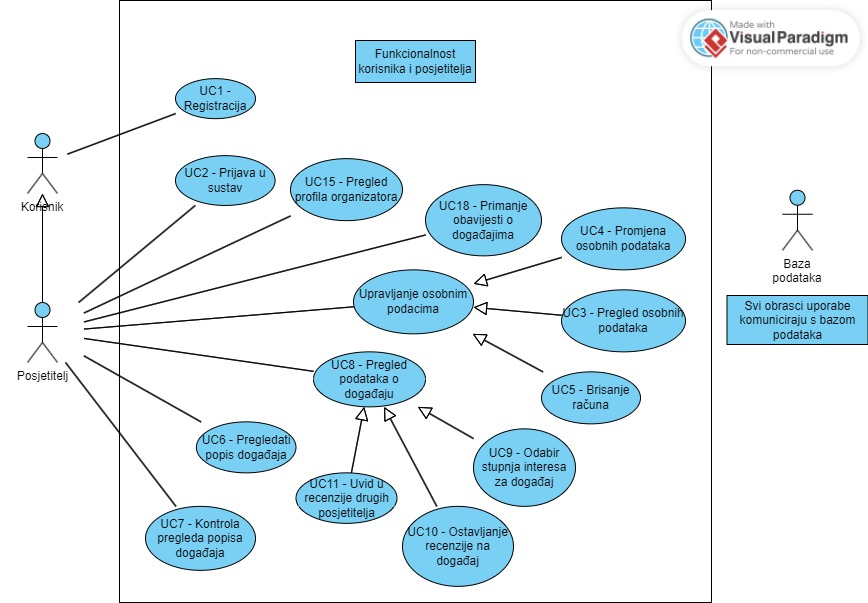
\includegraphics[width=1\textwidth]{dijagrami/obrazac_funkcionalnost_posjetitelja.jpg}
						\caption{Dijagram obrasca uporabe, funkcionalnost posjetitelja}
					\label{fig:my_image}
					\end{figure}
					
					\begin{figure}[htbp]
						\centering
						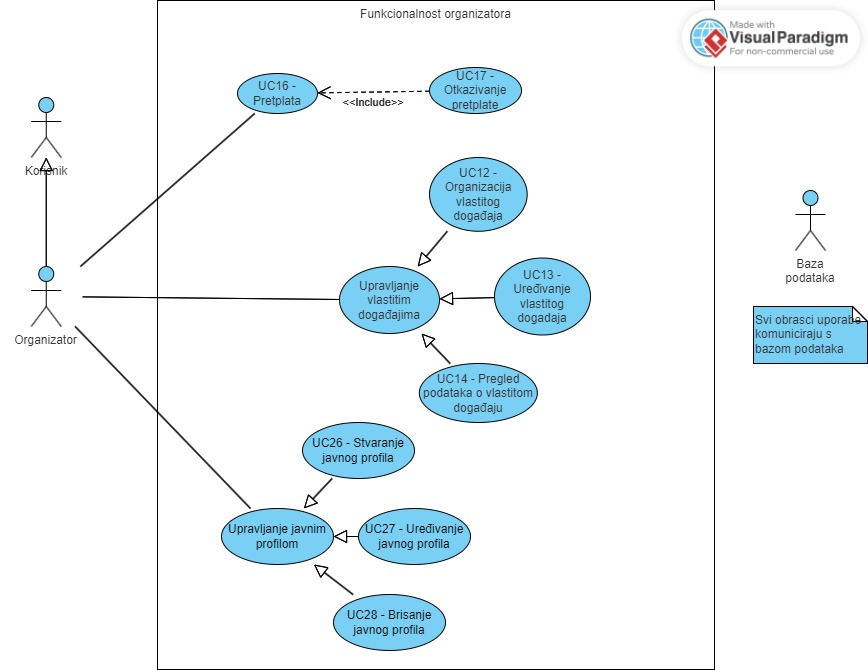
\includegraphics[width=1\textwidth]{dijagrami/obrazac_funkcionalnost_organizatora.jpg}
						\caption{Dijagram obrasca uporabe, funkcionalnost organizatora}
					\label{fig:my_image}
					\end{figure}

					\begin{figure}[htbp]
						\centering
						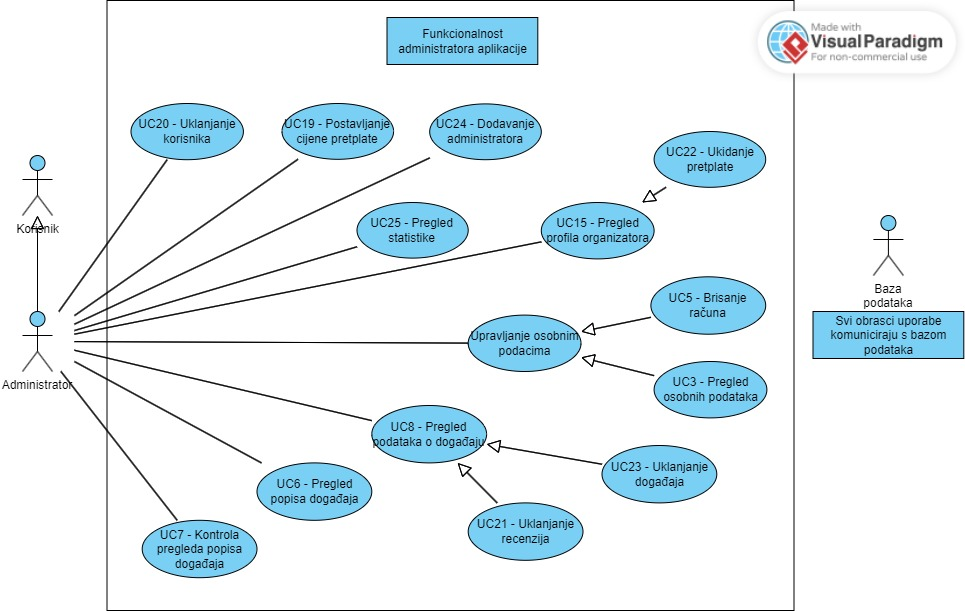
\includegraphics[width=1\textwidth]{dijagrami/obrazac_funkcionalnost_administratora.jpg}
						\caption{Dijagram obrasca uporabe, funkcionalnost administratora}
					\label{fig:my_image}
					\end{figure}


				\eject
				\pagebreak
			
			\newpage
			\subsection{Sekvencijski dijagrami}
				%\subsubsection{Obrazac uporabe UC1-Registracija}
        \noindent \textbf{UC1-Registracija}
				%\textbf{\textit{dio 1. revizije}}\\
				
				%\textit{Nacrtati sekvencijske dijagrame koji modeliraju najvažnije dijelove sustava (max. 4 dijagrama). Ukoliko postoji nedoumica oko odabira, razjasniti s asistentom. Uz svaki dijagram napisati detaljni opis dijagrama.}
				
				Korisnik odabire opciju za registraciju. Poslužitelj mu vraća obrazac za ispunjavanje osobnih podataka. 
        Nakon unosa poslužitelj provjerava je li korisnik unio neki podatak u neispravnom formatu ili je pružio neispravnu adresu e-pošte. 
        Nakon toga komunicira s bazom podataka kako bi provjerio da li slučajno postoji isto korisničko ime kao ono koje korisnik namjerava unijeti. 
        Ukoliko korisničko ime nije zauzeto i ostali podaci su ispravni dodaje se novi korisnički račun u bazu podataka i korisniku se vraća potvrda o uspješnoj registraciji. 
        U suprotnom prikazuje se početna stranica za registraciju.
				
				\newpage

        \begin{figure}[htbp]
          \centering
          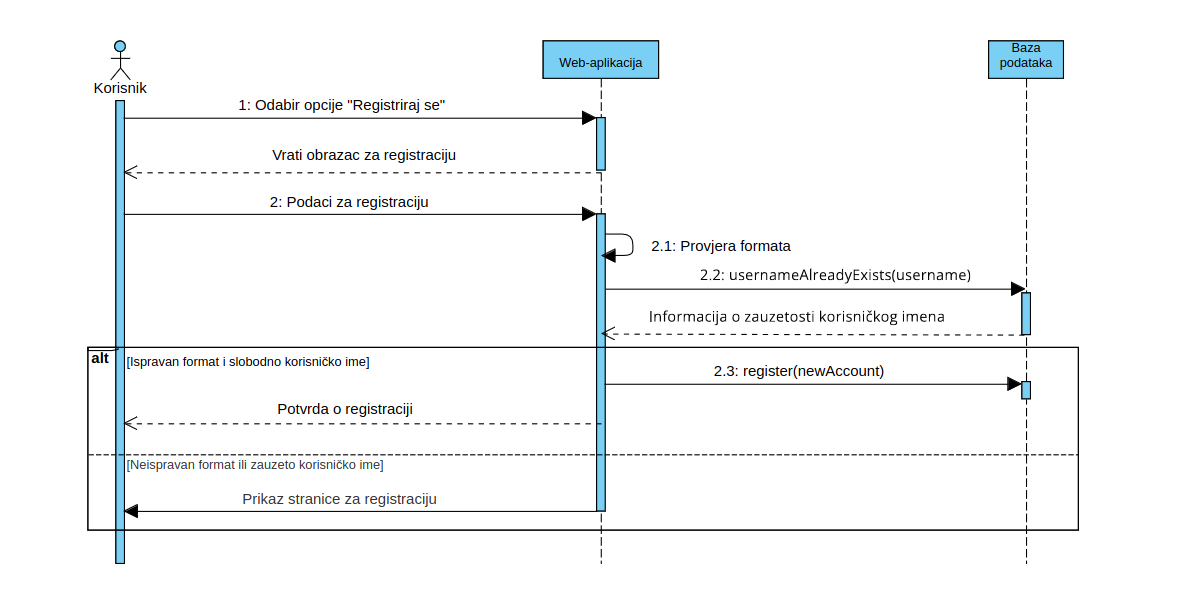
\includegraphics[width=1\textwidth]{dijagrami/uc1_registracija.png}
          \caption{Sekvencijski dijagram za UC1}
        \label{fig:my_image}
        \end{figure}


				\noindent \textbf{UC10 - Ostavljanje recenzije na dogadaj}

				\noindent Posjetitelj šalje zahtjev za prikaz događaja na kojima je bio 
				(kartica "Moji događaji") kako bi mogao odabrati događaj na kojem
				želi ostaviti recenziju. Poslužitelj dohvaća takve događaje iz baze podataka
				i prikazuje ih. Odabirom događaja, poslužitelj dohvaća podatke o događaju
				i prikazuje ih posjetitelju. Posjetitelj odabire opciju "Ostavi recenziju"
				te mu se prikazuje obrazac za ostavljanje recenzije. Posjetitelj unosi
				ocjenu i komentar te odabire opciju "Potvrdi recenziju". Poslužitelj
				sprema recenziju u bazu podataka i prikazuje poruku o uspješnom ostavljanju
				recenzije. Ako posjetitelj nije odabrao ocjenu ili nije unio komentar,
				prikazuje se poruka o neispravno popunjenom obrascu. Ako se posjetitelj
				predomisli, može odabrati opciju "Poništi" te se vraća na stranicu s
				podacima o događaju.

				\begin{figure}[htbp]
					\centering
					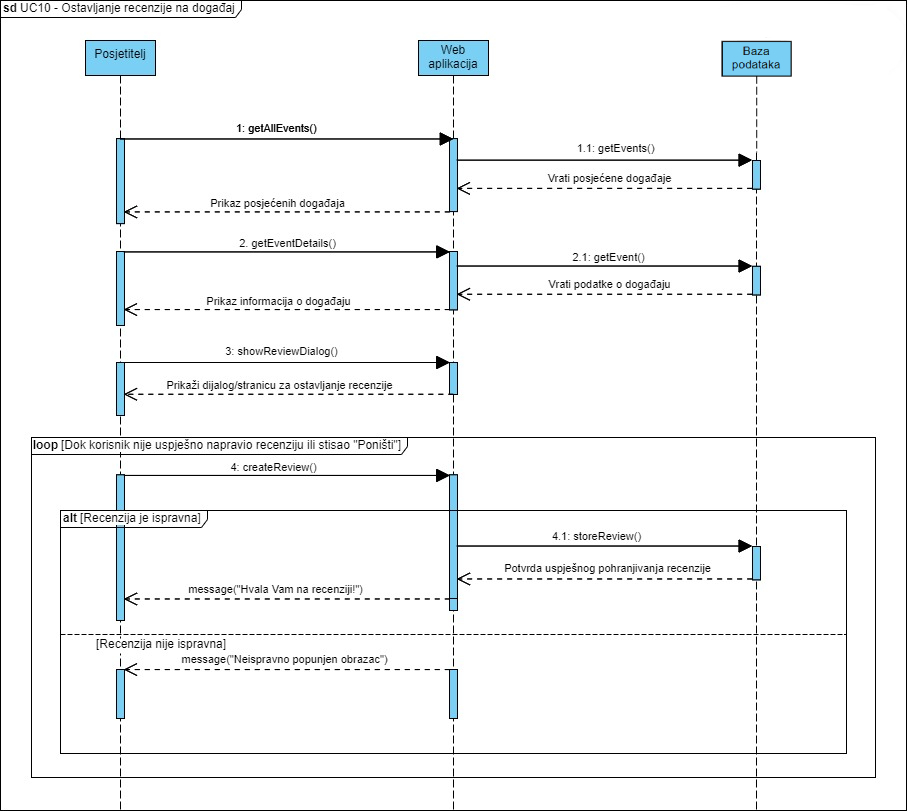
\includegraphics[width=1\textwidth]{dijagrami/seq_diagram_review.jpg}
					\caption{Sekvencijski dijagram za UC10}
				\label{fig:my_image}
				\end{figure}

     \eject
	
		\section{Ostali zahtjevi}
			%\textbf{\textit{dio 1. revizije}}\\
			% \textit{Nefunkcionalni zahtjevi i zahtjevi domene primjene dopunjuju funkcionalne zahtjeve. Oni opisuju \textbf{kako se sustav treba ponašati} i koja \textbf{ograničenja} treba poštivati (performanse, korisničko iskustvo, pouzdanost, standardi kvalitete, sigurnost...). Primjeri takvih zahtjeva u Vašem projektu mogu biti: podržani jezici korisničkog sučelja, vrijeme odziva, najveći mogući podržani broj korisnika, podržane web/mobilne platforme, razina zaštite (protokoli komunikacije, kriptiranje...)... Svaki takav zahtjev potrebno je navesti u jednoj ili dvije rečenice.}
			 
			\begin{itemize}
				\item Sustav treba omogućiti rad više korisnika u stvarnom vremenu
				\item Korisničko sučelje i sustav moraju podržavati hrvatsku abecedu (dijakritičkeznakove) pri unosu i prikazu tekstualnog sadržaja
				\item Izvršavanje dijela programa u kojem se pristupa bazi podataka ne smije trajati duže od nekoliko sekundi
				\item Sustav treba biti implementiran kao web aplikacija koristeći objektno orijentirane jezike
				\item Neispravno korištenje korisničkog sučelja ne smije narušiti funkcionalnost i rad sustava
				\item Sustav treba biti jednostavan za korištenje, korisnici se trebaju znati koristiti korisničkim sučeljem bez opširnih uputa
				\item Nadogradnja sustava ne smije narušavati postojeće funkcionalnosti sustava
				\item Sustav kao valutu koristi Euro
				\item Veza s bazom podataka mora biti kvalitetno zaštićena, brza i otporna na vanjske greške
				\item Pristup sustavu mora biti omogućen iz javne mreže pomoću HTTPS
			\end{itemize} 
			 
	